\documentclass[a4paper,11pt,captions=nooneline,parskip=half]{scrreprt}
\usepackage{IO-SEA_Report}

%%%%%%%%%%%%%%%%%%%%%%%%%%%%%%%%%%%%%%%%
% global configuration                 %
%%%%%%%%%%%%%%%%%%%%%%%%%%%%%%%%%%%%%%%%
\newcommand{\id}{D7.X}
\newcommand{\name}{The IO-SEA MAnifesto}
\newcommand{\version}{1.1}
\newcommand{\status}{Draft}
\newcommand{\authors}{Ph.~Deniel(CEA), B.~Writer(INST2))}
\newcommand{\contributors}{A.~Contributor (INST3)}
\newcommand{\reviewerI}{A.~Reviewer~(INST4)}
\newcommand{\reviewerII}{B. Reviewer~(INST5)}
\newcommand{\website}{\url{https://www.iosea-project.eu/}}
\newcommand{\leadingzero}[1]{\ifnum #1<10 0\the#1\else\the#1\fi}
%\newcommand{\dateI}{31.07.2021}
\newcommand{\dateI}{\today}  %%%% use today's date until done

\newcommand{\keywords}{IO-SEA, HPC, Exascale, Software}

\hypersetup{pdftitle={IO-SEA \id: \name},pdfauthor={\authors},pdfkeywords={\keywords}}

%%%%%%%%%%%%%%%%%%%%%%%%%%%%%%%%%%%%%%%%%%%%%%%%%%%%%%%
%here we input the glossary data %%%%%%%%%%%%%%%%%%%%%%
%%% This must be before the \begin{document} %%%%%%%%%%
%%%%%%%%%%%%%%%%%%%%%%%%%%%%%%%%%%%%%%%%%%%%%%
%%%%%%%% place glossary entries below %%%%%%%%%


%%%% NOTE!!!!!!!!!!!!

 %%% I think you MUST mark a glossary term with \Gls{} in the text for it to appear in the glossary


\glssetwidest[0]{blahblahblahblah}

\newglossaryentry{Hercule}{
    name=Hercule,
    description={Parallel I/O and data management library developed at CEA}
}

\newglossaryentry{AMR}{
    name=AMR,
    description={Adaptive Mesh Refinement} 
}

\newglossaryentry{RAMSES}{
    name=RAMSES,
    description={Code to model astrophysical systems, featuring self-gravitating, magnetised, compressible, radiative fluid flow, using AMR technique.}
}

\newglossaryentry{JSC}{
    name=JSC,
    description={The J\"{u}lich Supercomputing Centre at the Forschungszentrum  J\"{u}lich is one of the IO-SEA partners}
}
\newglossaryentry{FZJ}{
    name=FZJ,
    description={Forschungszentrum J\"{u}lich, in J\"{u}lich, Germany, is one of the largest research centres in Europe and a member of the Helmholtz Association}
}

\newglossaryentry{LQCD}
{
    name=LQCD,
    description={Lattice quantum-chromodynamics is a numerical framework for calculating physical properties of hadrons, composite particles composed of quarks}
}

\newglossaryentry{TSMP}
{
    name=TSMP,
    description={Terrestrial System Modelling Platform is an open source scale-consistent, highly modular, massively parallel regional Earth system model}
}

\newglossaryentry{COSMO}
{
    name=COSMO,
    description={Consortium for Small-scale Modeling}
}

\newglossaryentry{CLM}
{
    name=CLM,
    description={Community Land Model}
}

\newglossaryentry{CLI}
{
    name=CLI,
    description={Command Line Interface}
}

\newglossaryentry{ParFlow}
{
    name=ParFlow,
    description={A physically-based and spatially distributed hydrological model solving surface and subsurface flows in a massively parallel computational framework}
}
\newglossaryentry{OASIS3-MCT}
{
    name=OASIS,
    description={OASIS3-MCT is a software allowing synchronized exchanges of coupling information between numerical codes representing different components of the Earth System}
}
\newglossaryentry{MPMD}
{
    name=MPMD,
    description={Multiple Program Multiple Data}
}

\newglossaryentry{IFS}
{
    name=IFS,
    description={Integrated Forecasting System, ECMWF's operational weather forecasting system}
}
\newglossaryentry{MARS}
{
    name=MARS,
    description={The Meteorological Archival and Retrieval System is ECMWF's perpetual archive service}
}
\newglossaryentry{RAM}
{
    name=RAM,
    description={Random Access Memory  is memory optimised for random access, often by a compute device}
}

\newglossaryentry{NetCDF}
{
    name=NetCDF,
    description={NETwork Common Data Form is a community standard, machine-independent data format that support the creation, access, and sharing of array-oriented scientific data. It is extensively used in Earth system modelling}
}
\newglossaryentry{NVRAM}
{
    name=NVRAM,
    description={Non-volatile \Gls{RAM} is \Gls{RAM} that does not lose the stored information after a short time without constant refreshing}
}

\newglossaryentry{MSA}
{
    name=MSA,
    description={Modular Supercomputing Architecture}
}
\newglossaryentry{DA}
{
    name=DA,
    description={Data Assimilation}
}
\newglossaryentry{CUDA}{
    type=\acronymtype,
    name=CUDA,
    description={The Compute Unified Device Architecture is a parallel computing platform as well as an API that allows for the communication with certain types of graphics-processing units}
}
\newglossaryentry{CPU}
{
    name=CPU,
    description={Central Processing Unit}
}
\newglossaryentry{GPU}
{
    name=GPU,
    description={Graphics Processing Unit}
}
\newglossaryentry{SDLTS}
{
    name=SDLTS,
    description={Simulation and Data Laboratory: Terrestrial Systems}
}
\newglossaryentry{ECMWF}
{
    name=ECMWF,
    description={European Centre for Medium-Range Weather Forecasts}
}
\newglossaryentry{ParTec}
{
    name=ParTec,
    description={ParTec is one of the leading SMEs in the HPC domain in Europe}
}
\newglossaryentry{IT4I}
{
    name=IT4I,
    description={IT4Innovations National Supercomputing Centre at VSB Technical University of Ostrava, Czech Republic}
}
\newglossaryentry{ATOS}
{
    name=ATOS,
    description={ATOS is Europe's largest digital services deliverer}
}
\newglossaryentry{Eviden}
{
    name=Eviden,
    description={Eviden, formerly ATOS, is Europe's largest digital services deliverer}
}
\newglossaryentry{CEA}
{
    name=CEA,
    description={The French Alternative Energies and Atomic Energy Commission}
}
\newglossaryentry{PDAF}
{
    name=PDAF,
    description={Parallel Data Assimilation Framework}
}

\newglossaryentry{CEITEC}
{
    name=CEITEC,
    description={Central European Institute of Technology, Masaryk University, Brno, Czech Republic}
}


\newglossaryentry{MU}
{
    name=MU,
    description={Masaryk University, Brno, Czech Republic}
}


\newglossaryentry{iRODS}
{
    name=iRODS,
    description={Integrated Rule-Oriented Data System}
}

\newglossaryentry{PID}
{
    name=PID,
    description={Persistent Identifier}
}
\newglossaryentry{HSM}
{
    name=HSM,
    description={Hierarchical Storage Management}
}
\newglossaryentry{S3}
{
    name=S3,
    description={Amazon's Simple Storage Service: HTTP-based protocol to access data. Initially developed by Amazon, it generalisation made it a de facto standard for data access in cloud services}
}
\newglossaryentry{TCO}
{
    name=TCO,
    description={Total Cost of Ownership}
}
\newglossaryentry{SSD}
{
    name=SSD,
    description={Solid State Drive}
}
\newglossaryentry{HDD}
{
    name=HDD,
    description={Hard Drive Disk}
}
\newglossaryentry{HTTP}
{
    name=HTTP,
    description={HyperText Transfer Protocol: common Internet protocol to access web pages or download files}
}
\newglossaryentry{NVMe}
{
    name=NVMe,
    description={Non-Volatile Memory Express}
}
\newglossaryentry{NVMe-oF}
{
    name=NVMe-oF,
    description={NVM Express over Fabrics}
}
\newglossaryentry{Swift}
{
    name=Swift,
    description={Object-based interface of the OpenStack suite}
}
\newglossaryentry{POSIX}
{
    name=POSIX,
    description={Portable Operating System Interface is a family of standards specified by the IEEE Computer Society for maintaining compatibility between operating systems}
}
\newglossaryentry{API}{
    type=\acronymtype,
    name=API,
    description={An Application Programming Interfaces (API) allows software to communicate with other software which support the same API}
}
\newglossaryentry{DASI}{
    name=DASI,
    description={Data Access and Storage Interface developed in Work Package 5}
}

\newglossaryentry{SLURM}{
    name=SLURM,
    description={SLURM is an open-source cluster-management and job-scheduling system}
}

\newglossaryentry{JUBE}{
    type=\acronymtype,
    name=JUBE,
    description={The J\"{U}lich Benchmarking Environment is a script based framework to easily create benchmark sets, run those sets on different computer systems and to evaluate the results}
}

\newglossaryentry{CI/CD}{
    name=CI/CD,
    description={Continuous Integration/Continuous Deployment is an automated system for the testing, integration and deployment of software}
}

\newglossaryentry{CM}{
    name=CM,
    description={Cluster Module - the general purpose compute module of the DEEP System}
}

\newglossaryentry{ESB}{
    name=ESB,
    description={Extreme Scale Booster - module of the DEEP System focused on compute intensive applications with high scalability}
}

\newglossaryentry{DAM}{
    name=DAM,
    description={Data Analytics Module of the DEEP System focused on data-intensive applications}
}

\newglossaryentry{SSSM}{
    name=SSSM,
    description={Scalable Storage Service Module - conventional, spinning-disk-based storage module of the DEEP System}
}

\newglossaryentry{AFSM}{
    name=AFSM,
    description={The All-Flash Storage Module is a purely flash-based storage module of the \Gls{DEEP} system}
}

\newglossaryentry{Kronos}{
    name=Kronos,
    description={The ECMWF workload simulator}
}

\newglossaryentry{BDGS}{
    type=\acronymtype,
    name=BDGS,
    description={The Big Data Generator Suite efficiently generates scalable big data while employing data models derived from real data to preserve data veracity \cite{ming2013bdgs}}
}

\newglossaryentry{FDB}{
    name=FDB,
    description={Fields DataBase, the ECMWF meteorological object store}
}

\newglossaryentry{MPI}{
    type=\acronymtype,
    name=MPI,
    description={The Message Passing Interface is a common API for communication between tasks running on one or more computers}
}

\newglossaryentry{I/O}{
    type=\acronymtype,
    name=I/O,
    description={Input/Output is either a noun referring to the action of doing either input and/or output, generally either reading or writing memory, or is an adjective or adverb that describes that the following operation does input and/or output}
}

\newglossaryentry{DEEP}{
    type=\acronymtype,
    name=DEEP,
    description={The Dynamical Exascale Entry Platform (DEEP) is a multi-component project project to prepare for upcoming exascale HPC systems. The DEEP-SEA project is latest component of this project. It is also used to refer to the prototype developed in the DEEP projects based on context.}
}

\newglossaryentry{Git}{
    type=\acronymtype,
    name=Git,
    description={Git is a software for tracking changes to files that is often used amon programmers to coordinate work}
}
\newglossaryentry{GitLab}{
    type=\acronymtype,
    name=GitLab,
    description={GitLab is an open-source software-development--and--operations platform that uses Git to organize software development}
}

\newglossaryentry{OSU}{
    type=\acronymtype,
    name=OSU,
    description={The Ohio State University is a university in the state of Ohio in the United States of America}
}
\newglossaryentry{TCP}{
    type=\acronymtype,
    name=TCP,
    description={The Transmission Control Protocol  is one of the main communication protocols of the internet protocol}
}
\newglossaryentry{IB verbs}{
    type=\acronymtype,
    name=IB verbs,
    description={The API for communication using InfiniBand, a communication hardware}
}
\newglossaryentry{UCP}{
    type=\acronymtype,
    name=UCP,
    description={The Unified Communication Protocol is an API aimed at unifying different communication APIs, similiar in that sense to MPI}
}
\newglossaryentry{PSM2}{
    type=\acronymtype,
    name=PSM2,
    description={Performance Scaled Messaging 2 is the second generation of the PSM API for communication}
}
\newglossaryentry{NVLink}{
    type=\acronymtype,
    name=NVLink,
    description={NVLink describes the suite of tools for communicating between NVIDIA GPUs. It includes an API that requires physical NVLink bridges between GPUs to use}
}
\newglossaryentry{OMB}{
    type=\acronymtype,
    name=OMB,
    description={The Ohio State University (OSU) MicroBenchmarks is a suite of \Gls{MPI} benchmarks that has been extended to other communication \Glspl{API}}
}

\newglossaryentry{QIO}{
    type=\acronymtype,
    name=QIO,
    description={QCD Input/Output Applications Programmer Interface developed under the auspices of the U.S. Department of Energy Scientific Discovery through Advanced Computing (SciDAC) program}
}

\newglossaryentry{CHROMA}{
    type=\acronymtype,
    name=CHROMA,
    description={The Chroma software system for lattice QCD }
}

\newglossaryentry{ICHEC}{
    type=\acronymtype,
    name=ICHEC,
    description={Irish Centre for High-End Computing is the national HPC centre in Ireland.}
}
\newglossaryentry{FFT}{
    type=\acronymtype,
    name=FFT,
    description={The Fast Fourier Transform was originally an optimized algorithm proposed for Fourier transforming discrete data, nowadays it more commonly refers to a suite of better-optimized algorithms that perform said transform}
}

\newglossaryentry{SQL}{
    type=\acronymtype,
    name=SQL,
    description={The Structured Query Language  is a domain-specific language for accessing data in a \Gls{RDBMS} or in a \Gls{RDSMS}}
}

\newglossaryentry{RDBMS}{
    type=\acronymtype,
    name=RDBMS,
    description={A Relational-DataBase Management System (RDBMS) is a management system for relational databases}
}

\newglossaryentry{RDSMS}{
    type=\acronymtype,
    name=RDBMS,
    description={A Relational-Data--Stream Management System (RDSMS) is a management system for relational data streams}
}

\newglossaryentry{NoSQL}{
    type=\acronymtype,
    name=NoSQL,
    description={NOn relational \Gls{SQL}  databases are SQL databases that can efficiently handle huge amounts of unstructured rapidly changing data. NoSQL unlike SQL does not refer to a language and is generally an adjective}
}

\newglossaryentry{RED-SEA}{
    type=\acronymtype,
    name=RED-SEA,
    description={EuroHPC project focused on network solutions for exascale architectures}
}

\newglossaryentry{PCIe}{
    type=\acronymtype,
    name=PCIe,
    description={Peripheral Component Interconnect Express is a high-speed serial-bus expansion standard designed to unify and replace older standards}
}

\newglossaryentry{JURECA-DC}{
    type=\acronymtype,
    name=JURECA-DC,
    description={The J\"{U}lich Research on Exascale Cluster Architectures -- Date Centre  module is one of the modules of the J\"{U}lich Research on Exascale Cluster Architectures (JURECA) system}
}

\newglossaryentry{JUWELS}{
    type=\acronymtype,
    name=JUWELS,
    description={The J\"{U}lich Wizard for European Leadership Science is one of the super computers at \Gls{JSC}}
}

\newglossaryentry{HPL}{
    type=\acronymtype,
    name=HPL,
    description={The High Performance \Gls{LINPACK} is a performant software package for solving linear system}
}

\newglossaryentry{LINPACK}{
    type=\acronymtype,
    name=LINPACK,
    description={LINPACK is a software package for solving linear systems}
}

\newglossaryentry{FLOPS}{
    type=\acronymtype,
    name=FLOPS,
    description={FLoating-point OPerations per Second (FLOPS) is the number of floating-point operations achieved in a second}
}

\newglossaryentry{SEA}{
    type=\acronymtype,
    name=SEA,
    description={The Software/Solutions for Exascale Architectures  project is a joint combination of three separate projects \Gls{DEEP}-, IO-, and RED-SEA}
}

\newglossaryentry{HBM2}{
    type=\acronymtype,
    name=HBM2,
    description={The second generation of High Bandwidth Memory  using synchronous dynamic random-access memory stacked in three dimensional space}
}

\newglossaryentry{TIFF}{
    type=\acronymtype,
    name=TIFF,
    description={The Tag Image File Format  is an image file format}
}

\newglossaryentry{HPC}{
    type=\acronymtype,
    name=HPC,
    description={High-Performance Computing}
}

\newglossaryentry{AI}{
    type=\acronymtype,
    name=AI,
    description={Artificial Intelligence}
}

\newglossaryentry{IOR}{
    type=\acronymtype,
    name=IOR,
    description={The Interleaved Or Random (IOR) benchmark is benchmark for \Gls{I/O}}
}

\newglossaryentry{MPI-I/O}{
    type=\acronymtype,
    name=MPI-I/O,
    description={\Gls{MPI} -- Input/Output is an extentsion to \Gls{MPI} for \Gls{I/O}}
}

\newglossaryentry{GPFS}{
    type=\acronymtype,
    name=GPFS,
    description={The General Parallel File System (GPFS) is an IBM developed high-performance clustered file system}
}

\newglossaryentry{Lustre}{
    type=\acronymtype,
    name=Lustre,
    description={Lustre is an open-source parallel file system}
}

\newglossaryentry{mdtest}{
    type=\acronymtype,
    name=mdtest,
    description={Included with the \Gls{IOR} benchmark, the mdtest benchmark is for benchmarking metadata creation}
}

\newglossaryentry{Linktest}{
    type=\acronymtype,
    name=Linktest,
    description={Linktest is a communication-API benchmark developed at \Gls{JSC}}
}

\newglossaryentry{FPGA}{
    type=\acronymtype,
    name=FPGA,
    description={Field-Programmable Gate Array}
}

\newglossaryentry{QCD}{
    type=\acronymtype,
    name=QCD,
    description={Quantum-ChromoDynamics (QCD)}
}

\newglossaryentry{GitLab Runner}{
    type=\acronymtype,
    name={GitLab Runner},
    description={A GitLab Runner is software that connects to GitLab servers for remote execution of CI/CD tasks}
}

\newglossaryentry{STREAM2}{
    type=\acronymtype,
    name={STREAM~2},
    description={A benchmark for measuring \Gls{CPU}-cache and \Gls{CPU}-to-\Gls{RAM} latencies and bandwidth}
}

\newglossaryentry{HPCG}{
    type=\acronymtype,
    name={HPCG},
    description={The High Performance Conjugate Gradient benchmark is a benchmark based on a conjugate-gradient kernel}
}

\newglossaryentry{HMC}{
    type=\acronymtype,
    name={HMC},
    description={The Hamiltonian Monte Carlo algorithm (originally known as hybrid Monte Carlo) is a Markov chain Monte Carlo method for obtaining a sequence of random samples which converge to being distributed according to a target probability distribution for which direct sampling is difficult}
}
\newglossaryentry{WDF}{
    type=\acronymtype,
    name={WDF},
    description={The workflow description file is a YAML configuration file describing ephemeral services and steps invoked in a workflow}
    }

\newglossaryentry{WFM}{
    type=\acronymtype,
    name={WFM},
    description={The IO-SEA Workflow Manager starts ephemeral storage services, and runs workflow steps in the IO-SEA storage environment.
    %\fxnote{ Maybe polish the WFM definition.}
    }
    }
\newglossaryentry{SBB}{
    type=\acronymtype,
    name={SBB},
    description={Smart Burst Buffer is a hardware
accelerator that can be included in the I/O data
path and accelerate I/O on specific files for
targeted applications. Offered as an IO-SEA ephemeral service.
}}

\newglossaryentry{IOI}{
    type=\acronymtype,
    name={IOI},
    description={The IO Instrumentation tool collects I/O-related metrics and provides  diagnostic information about workflow read and wrinte operations}
}
\newglossaryentry{NFS}{
    type=\acronymtype,
    name={NFS},
    description={Network File System, a file system allowing to share files between many nodes over a TCP/IP network}
}
\newglossaryentry{mmap}{
    type=\acronymtype,
    name={mmap},
    description={mmap is a POSIX-compliant Unix system call that maps files or devices into memory}
}


\newglossaryentry{PFB}{
    type=\acronymtype,
    name={PFB},
    description={ParFlow Binary format is a binary file format which is used to store ParFlow grid data}
}


\newglossaryentry{NCL}{
    type=\acronymtype,
    name={NCL},
    description={The NCAR Command Language is an open source interpreted language, designed specifically for scientific data processing and visualization}
}


\makeglossaries

%%%%%%%%%%%%%%%%%%%%%%%%%%%%%%%%%%%%%%%%
% document body                        %
%%%%%%%%%%%%%%%%%%%%%%%%%%%%%%%%%%%%%%%%
\begin{document}
	\hypersetup{pageanchor=false}
	%%%%%%%%%%%%%%%%%Titlepage.tex included here %%%%%%%%%%%%%%%%%%%
	\begin{titlepage}
	\thispagestyle{empty}
	\begin{center}
		\begin{figure}[h!]
			\centering
			
\includegraphics[width=0.5\textwidth]{Preamble/io-sea-logo}
		\end{figure}

		\vspace*{3\baselineskip}

		{\large\textbf{EuroHPC-01-2019}}

		\vspace*{2\baselineskip}

		\begin{figure}[h!]
			\centering
			
\includegraphics[width=0.2\textwidth]{Preamble/flag_yellow}
		\end{figure}

		\vspace*{2\baselineskip}

		{\Large\textbf{IO-SEA}}

		\vspace*{1.5\baselineskip}

		{\Large\textbf{IO -- Software for Exascale Architectures}}\\
		{\textbf{Grant Agreement Number: 955811}}

		\vspace*{1.5\baselineskip}

		{\Large\textbf{\id}}\\
		{\large\textbf{\name}}

		\vspace*{1.5\baselineskip}

		{\large\textit{\textbf{\status}}}\\
	\end{center}

	\vspace*{4\baselineskip}

	\begin{tabularx}{\textwidth}{l >{\raggedright\let\\\tabularnewline}X}
		\textbf{Version:} & \version \\
		\textbf{Author(s):} & \authors \\
		\textbf{Contributor(s):} & \contributors \\
		\textbf{Date:} & \dateI
	\end{tabularx}
 
	\begin{tikzpicture}[overlay]
		\def\pt{\paperwidth/3}
		\def\plm{1in}
		\def\ptm{1in}
		\def\phs{.76\paperheight}
		\def\phe{.8\paperheight}
		\fill[color=ioseared] (-\plm, \phs) rectangle (-\plm+\pt, \phe);
		\fill[color=ioseagreen] (-\plm+\pt, \phs) rectangle (-\plm+2\pt, \phe);
		\fill[color=ioseablue] (-\plm+2\pt, \phs) rectangle (-\plm+3\pt, \phe);

		\draw[color=ioseagrey] (-\plm, \phs) rectangle (-\plm+\pt, \phe);
		\draw[color=ioseagrey] (-\plm+\pt, \phs) rectangle (-\plm+2\pt, \phe);
		\draw[color=ioseagrey] (-\plm+2\pt, \phs) rectangle (-\plm+3\pt, \phe);
	 \end{tikzpicture}
\end{titlepage}

	\hypersetup{pageanchor=true}
	\pagenumbering{arabic}

	%%%%%%%%%%%% Infosheet.tex included here %%%%%%%%%%%%%%
	\section*{Project and Deliverable Information Sheet}
\addcontentsline{toc}{chapter}{Project and Deliverable Information Sheet}
\begin{tabularx}{\textwidth}{| p{2.5cm} | p{4cm} | >{\raggedright\let\\\tabularnewline}X |}
 \hline
 \textbf{IO-SEA} & \textbf{Project ref. No.:} & 955811 \\ \cline{2-3}
 \textbf{Project} & \textbf{Project Title:} & IO -- Software for Exascale Architectures \\ \cline{2-3}
 & \textbf{Project Web Site:} & \website \\ \cline{2-3}
 & \textbf{Deliverable ID:} & \id \\ \cline{2-3}
% & \textbf{Deliverable Nature:} & Report / Other / DEM / DEC \\ \cline{2-3}
 & \textbf{Deliverable Nature:} & Report \\ \cline{2-3}
 & \textbf{Deliverable Level:} & \textbf{Contractual Date of Delivery:} \\
 & PU $^{*}$ & 31 / December / 2021\\ \cline{3-3}
 & & \textbf{Actual Date of Delivery:} \\
 & & ?? / December / 2021\\ \cline{2-3}
 & \textbf{EC Project Officer:} & Daniel Opalka \\
 \hline
\end{tabularx}

{\small $^{*} - $ The dissemination levels are indicated as follows: \textbf{PU} - Public, \textbf{PP} - Restricted to other participants (including the Commissions Services), \textbf{RE} - Restricted to a group specified by the consortium (including the Commission Services), \textbf{CO} - Confidential, only for members of the consortium (including the Commission Services).}

\vfill

\section*{Document Control Sheet}
\addcontentsline{toc}{chapter}{Document Control Sheet}
\begin{tabularx}{\textwidth}{| p{2.5cm} | p{4cm} | >{\raggedright\let\\\tabularnewline}X |}
 \hline
 & \multicolumn{2}{l |}{\textbf{Title:}  \name}\\ \cline{2-3}
 \textbf{Document} & \multicolumn{2}{l |}{\textbf{ID:}  \id}\\ \cline{2-3}
 & \textbf{Version:}  \version & \textbf{Status:}  \status\\ \cline{2-3}
 & \multicolumn{2}{l |}{\textbf{Available at:}  \website}\\ \cline{2-3}
 & \multicolumn{2}{l |}{\textbf{Software Tool:}  \LaTeX}\\ \cline{2-3}
 & \multicolumn{2}{l |}{\textbf{File(s):} IO\_SEA\_Manifesto.pdf}\\
 \hline
 & \textbf{Written by:} & \authors \\ \cline{2-3}
 \textbf{Authorship} & \textbf{Contributors:} & \contributors \\ \cline{2-3}
 & \textbf{Reviewed by:} & \reviewerI \\
 & & \reviewerII \\ \cline{2-3}
 & \textbf{Approved by:} & Exec Board/WP7 Core Group\\
 \hline
\end{tabularx}

	\clearpage
	%%%%%%%%%%%%%%%%%%%%%%%%%%%%%%%%%%%%%%%%%%%%%%%%%%%%%%%%%%%%%%%%%
	%%%%%%%%%%%%%  Document Status Sheet inlined here %%%%%%%%%%%%%
	\section*{Document Status Sheet}
	\addcontentsline{toc}{chapter}{Document Status Sheet}
	\begin{tabularx}{\textwidth}{| l | l | l | >{\raggedright\let\\\tabularnewline}X |}
		\hline
		\textbf{Version} & \textbf{Date} & \textbf{Status} & \textbf{Comments}\\
		\hline
		0.1 & XX.XX.2022 & Outline approved & complete?\\
				\hline
		0.9 & XX.XX.2022 & Draft ready for internal review & \\
		\hline
		1.0 & XX.XX.2022 & 1st internal review complete & \\
        \hline
        		1.1 & XX.XX.2022 & post-1st-review edits complete & \\
        \hline
		2.0 & XX.XX.2022 & final draft ready for EU submission & \\
		\hline
	\end{tabularx}
	\vfill
	\begin{tabularx}{\textwidth}{| l  | >{\raggedright\let\\\tabularnewline}X |}
		\hline
		\textbf{Section} & \textbf{Status} \\
		\hline
		Executive summary & {\color{red} in progress }\\ 
		\hline
		Introduction & {\color{orange} Ready for proofreading}\\
		\hline
		\hline
		Some Chapter & {\color{blue} Proofread}\\
		\hline
		\hline
		Another Chapter & {\color{green}Ready for review}\\
		
		\hline
		\hline
		Summary & {\color{red} In progress}\\
		\hline
	\end{tabularx}
	\clearpage

	%%%%%%%%%%%%%%%% Document_Keywords.tex included here %%%%%%%%
	\section*{Document Keywords}
\begin{tabularx}{\textwidth}{| p{3cm} | >{\raggedright\let\\\tabularnewline}X |}
  \hline
  \textbf{Keywords:} & \keywords\\
  \hline
\end{tabularx}

\vfill

\begin{framed}
  \textbf{Copyright notice:}

  \bigskip

  \textcopyright\,2021-2024 IO-SEA Consortium Partners. All rights
  reserved. This document is a project document of the IO-SEA
  Project. All contents are reserved by default and may not be
  disclosed to third parties without written consent of the IO-SEA
  partners, except as mandated by the European Commission contract
  955811 for reviewing and dissemination purposes.

  All trademarks and other rights on third party products mentioned in
  this document are acknowledged as own by the respective holders.
\end{framed}

	\clearpage
	\tableofcontents
	\iftotalfigures
	\clearpage
	\phantomsection\addcontentsline{toc}{chapter}{\listfigurename}
	\listoffigures
	\fi
	\iftotaltables
	\clearpage
	\phantomsection\addcontentsline{toc}{chapter}{\listtablename}
	\listoftables
	\fi
	%uncomment for list of fixes
	\listoffixmes
	
	\chapter*{Executive Summary}
\addcontentsline{toc}{chapter}{Executive Summary}

%Also adapt the Titlepage and Infosheet as necessary\\
%{\color{blue} These are located in {\ttfamily Preamble/}}

This document aims to be an annex to the last WP7 deliverable. It reminds the objectives and goals of the IO-SEA
project at the tile the project was submitted in late~2019 and early~2020. It then describes  the works 
done during the project and the related outcomes. From this perspective, this document then explains the topics that could be developed if someone wants to leverage the IO-SEA project for a later use in another project. 

\paragraph{}
In some ways, this "IO-SEA manifesto" is a "testament" too, it clearly defines what you can inherit fron IO-SEA
and the benefits you can get by using the provided results and outcomes.  
	\chapter{Introduction}\label{sec:introduction}
%
%{\color{blue} Located in {\ttfamily Introduction.tex}}

The IO-SEA project is very close to its end at the time we write this document. This document is the "IO-SEA" 
manifesto, it aims to give all the keys to someone willing to leverage the outcomes of the IO-SEA project for
setting up a new project.

\paragraph{}
This approach is done via several steps. First, we will describe the original goals and ambitions of the project
as it was set up in late~2019 and early-2020. Since that time, the project was accomplished and it produced real
outcomes. 

The Devil is in the details and a few features, that have not been foreseen as the project was prepared, exists. 
They are peripheral and do not impact the run of the IO-SEA software stack that could easily work around it. 

On the other hand, some unexpected results arrived on the table, and they are actual benefits to be leveraged
and potentially reused in later projects. 

\paragraph{}
This document will gather all of this aspects, showing them in a short and synthetic manner. It is kind of 
"testament" or "manifesto", with the ambitions of giving the IO-SEA software stack keys to everyone willing
to use some elements from IO-SEA for other applications and projects. 


	\label{part:firstpart}
	\chapter{Goals of the IO-SEA project}\label{chap:goals}
%%{\color{blue} Located in {\ttfamily Goals.tex}}\\

This chapter is an overview of the ambition of the IO-SEA project as presented and exposed in the proposal.
This view is more than three years old. It highlights the main topics that drove the development of the IO-SEA
software stack. We should first quickly summarize them. 

\paragraph{}
Let's take a few seconds and have a look at the backmirror. The very first paragraph of the IO-SEA proposal 
clearly states the ambitions and goals of the project, which are described at this:

\begin{quotation}
IO-SEA aims to provide a novel data management and storage platform for exascale computing based on hierarchical
storage management (HSM) and on-demand provisioning of storage services. The platform will efficiently make use
of storage tiers spanning NVMe and NVRAM at the top all the way down to least active data stored with tape-based
technologies. System requirements are driven by data intensive use-cases, in a very strict co-design approach.
The concept of ephemeral data nodes and data accessors is introduced that allows users to flexibly operate the
system, using various well-known data access paradigms, such as POSIX namespaces, S3/Swift Interfaces, MPI-IO 
and other middleware, data formats and protocols. These ephemeral resources eliminate the problem of treating
storage resources as static and unchanging system components – which is not a tenable proposition for data
intensive exascale environments. The methods and techniques are applicable to exascale class data intensive
applications and workflows that need to be deployed in highly heterogeneous computing environments.
\end{quotation}

\section{Highlights from the proposal}
In this section, we'll shortly remind the technological choices made in IO-SEA, as well as the underlying
concepts that drove the development of IO-SEA. 

\paragraph{}
The proposal then states which technologies and technical approaches to be fostered and leveraged:
\begin{itemize}
    \item object stores
    \item Hierarchical Storage Management (HSM)
    \item ephemeral services and scheduling
    \item IO Instrumentation and AI based analytics
    \item Co-design (this approach was later described by the deliverabmes from Work Package~\#1\cite{iosea-d1.1})
\end{itemize}

\paragraph{}
By taking in considerations those technologies, concepts and topcis to be advanced are then chosen:
\begin{itemize}
    \item Manage system scalability
    \item Manage data scalability
    \item Manage data heterogeneity
    \item Manage Data placement
\end{itemize}

\paragraph{}
In order to build an exascale IO software stack, the work done in IO-SEA was designed to be made following
those tracks:
\begin{itemize}
    \item as filesystem paradigm do not fit the scalability requirements and constraints from the Exascale era.
    The decided choice is to use object stores instead, as they do scale very well. This feature is achieved 
    due to the \textbf{C}reate \textbf{R}ead \textbf{U}pdate \textbf{D}elete (CRUD) semantics, which is simple 
    and compact. Because this semantics is very far from POSIX, which is much more complex, it is required to 
    build pieces of software, based on well identified design concepts. IO-SEA will develop those needed tools, 
    based on two mains ideas, which are \textit{datasets} and \textit{namespaces}. 
    
    \item Tapes is clearly the less expansive technology to be used to store data, making it to save money and 
    power. As IO-SEA has the ambition to manage tens or even hundreds of exabytes of data, using tapes can't
    reasonably be ignored, they clearly are to be used. Tapes have high capacity but they are really slow,
    especially when compared to modern storage media. As IO-SEA will involve HSM mechanisms, tapes are clearly
    a target for integrating this technology.
    
    \item High speed storage, including NVRAM and NVMe capable devices are at the oppositce side ofg the HSM 
    spectrum. As tapes are slow but offer high capacity, and are rather inexpensive, high speed storage is greedy
    in terms of energy consumption and are very expensive, and they do offer a very high bandwidth, a very small
    latency, as the cost of a reduced storage capability. As more classical storage, like rotating HDDs or
    standard SSDs, are inserted in this "storage spectrum", the question of comprehensive management of all
    devices, via an extended HSM implementation, becomes crucial.
    
    \item In order to perform an efficient HSM, it is necessary to collect information in order to have a 
    precise idea about the files to be managed. The first natural source for such information is naturally
    the end-user, who can add tags (or \textit{hints}) in order to help characterizing the pieces of data. Such
    information may be lacking, imprecise or erroneous. It could be necessary, most of the times, to automatize
    this process. In the IO-SEA software, tools are developed and/or leveraged in order to perform an as
    comprehensive as possible collection of information about the different pieces of data. The result of this
    precise IO instrumentation is then post-processed by AI analytics. This recommendation system automatically
    does the job of tagging the files with the correct related tags or hints. Those hints are required to 
    optimize the way the HSM is working and its efficiency. 
    
    \item as new data model are introduced, via HSM and object stores relying on datasets and namespaces 
    meta-structures, and as specific interfaces are developed (like ephemeral services), it makes sense to 
    look forward for new storage access paradigms. Within IO-SEA, the concept of Data and Access Storage 
    Interface (DASI) is introduced.  DASI will encourage applications to describe their data using meaningful semantics, on the one hand facilitating exploitation of those data, and on the other hand giving the opportunity for IO-SEA to optimise data placement given the intended access patterns.
    
    \item a direct consequence of the introduction of the concepts of datasets and namespaces are data nodes ans
    ephemeral services. As storage resourcves as clearly not infinite, batch environments today should schedule the usage of storage capacity and bandwidth. Ephemeral services, running on dedicated data nodes, themselves 
    closely acquainted with some compuofte nodes are introduced. Ephemeral servers may have different kinds or 
    flavors. They are IO server, spawned on demand and associated to a set of compute jobs, are working as
    dedicated IO servers for those compute jobs. It works both as an IO proxy server and as a bridge capable of
    translating the underlying object stores semantics to a different IO semantics. 
\end{itemize}

\paragraph{}
As a raw summary, the different aspects and features of the IO-SEA project may be gathered and
summarized under this schema depicted on the figure \ref{fig:iosea-nutshell} below. 
\begin{figure}[ht]
    \centering
    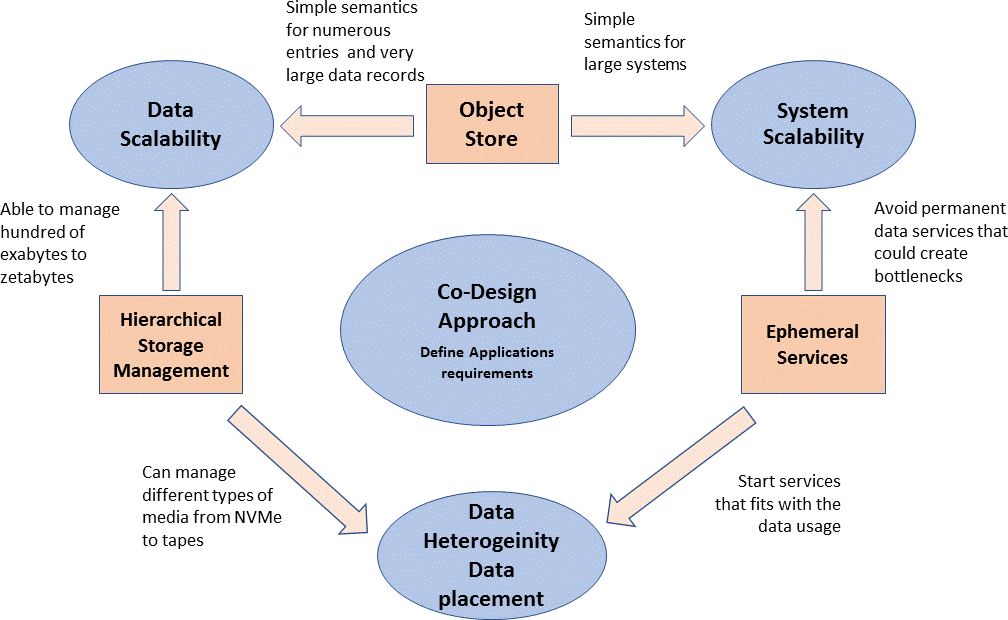
\includegraphics[width=\textwidth]{FIGS/IOsea.png}
    \caption[IO-SEA in a nutshell]{ How the technical choices and the technical challenges interact}
    \label{fig:iosea-nutshell}
\end{figure}

One the fundamental concept and underlying idea of IO-SEA is simple : storage is not an infinite resource, 
from both the capability or bandwidth point of view.   Sharing a restricted resource across a pool of users is
not a new problem and it has already been solved for sharing processors by batch schedulers like Slurm. In order
to use such resource managers, we will introduce two ideas to also handle storage as a shared resource:
\begin{itemize}
    \item Data accessors / ephemeral data services: data accessors are services that provide access to data for applications. For example, it can be a S3 or Swift server exposing objects, or a NFSv4 server that will show a namespace whose files will be connected to objects. Data accessors run as ephemeral services: a simulation workflow is associated with several data accessors; they are spawned at the beginning of the workflow and are dedicated to it. The ephemeral service will have no other clients than those running the simulation applications, and it will end when the workflow ends.
    
    \item Data nodes: ephemeral services need hardware to run on, those nodes are called ‘data nodes’. They have affinities with simulation nodes, which helps the resource manager choose data nodes that are close enough to compute nodes in terms of network location. Data nodes are a resource of the supercomputer, like compute nodes, and as such must be managed by a resource manager.
\end{itemize}

\section{IO-SEA, the MSA and the SEA legacy}

IO-SEA is not a standalone project, it is part of the "SEA legacy", a group of three projects funded under the
same EuroHPC JU call. The three projects target the Exascale era: the DEEP-SEA develops HPC middle-ware and
software, RED-SEA develops a new hardware and software network architecture while IO-SEA provides new storage
paradigm. All the projects go together and have strong interactions.

\begin{figure}[ht]
    \centering
    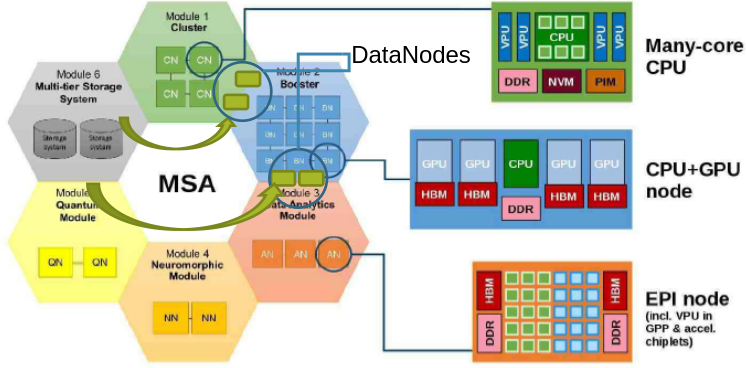
\includegraphics[width=\textwidth]{FIGS/MSA.png}
    \caption[The Modular Supercomputer Architecture]{ Data Nodes and Ephemeral Services within the MSA}
    \label{fig:msa}
\end{figure}

\paragraph{}
At the very core of this strong collaboration relies the Modular Supercomputing Architecture (MSA). MSA is made
of building blocks, or modules, each module having its own specific resources (for example GPU, or neuromorphic
processors). In this scope, it's quite natural to define a "IO module" which will hosts the IO-SEA data nodes
and run most of the server side IO-SEA software stack. With this approach, IO-SEA fits in the MSA as defined 
in figure \ref{fig:msa} . 


\section{The IO-SEA software components and their relationships}

This section describes how the different components of the IO-SEA infrastructure interact. The core of IO-SEA is
made of two object stores. Originally those object stores were the MOTR object store from Seagate, and Phobos an
open-source object store developed at CEA. The big picture of the IO-SEA software stack is described by figure
\ref{fig:iosea-sw-stack}. 

\begin{figure}[ht]
    \centering
    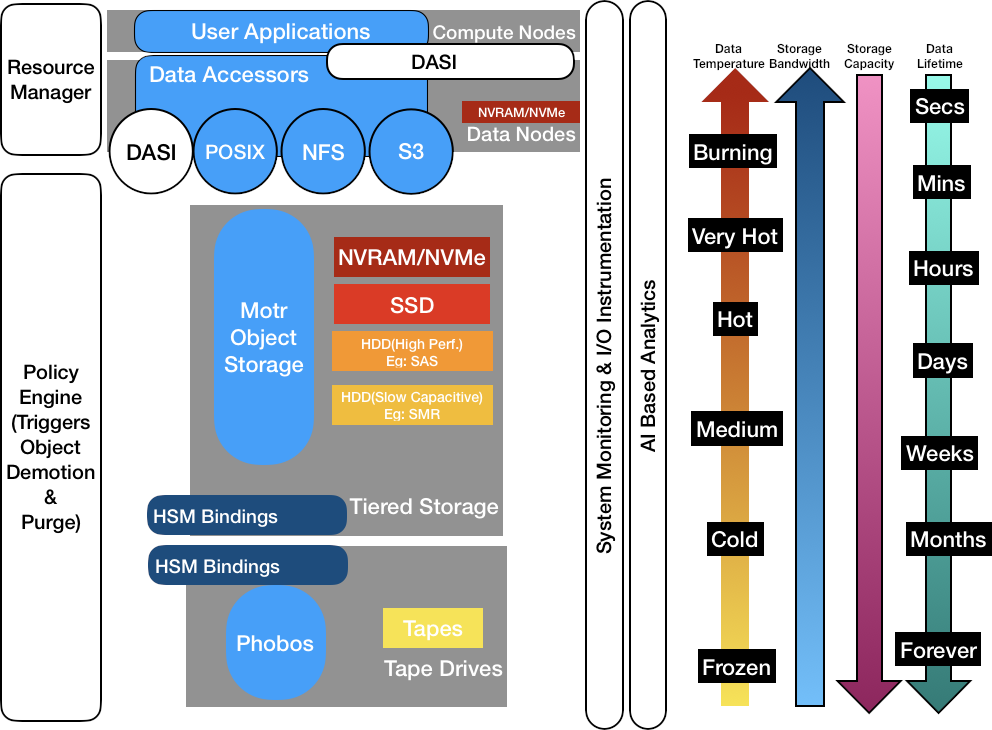
\includegraphics[width=\textwidth]{FIGS/iosea-swstack.png}
    \caption[IO-SEA software stack]{ The components of the IO-SEA software stack}
    \label{fig:iosea-sw-stack}
\end{figure}

Phobos is capable of dealing with tapes. MOTR is capable of dealing with a tiered storage stack, with
different kinds of disks. MOTR is HSM-ready (this is a direct outcome from the SAGE project). Those two object
stores inter-operates via a specifically designed HSM interface. In the run of the IO-SEA project, this component
gave birth to the HESTIA component, with a new and well defined API for HSM management.

\paragraph{}
On top of those HSM connected object stores, advanced interfaces are required, for object stores have very 
simple semantics\footnote{In particular, this makes it possible to scale object store very well}. For the 
majority of use cases, other interfaces are required to implement. For example, POSIX or NFS semantics are to 
be implemented. Dedicated servers are required, those are the ephemeral services. Original ephemeral services as
described in the original proposal includes NFS interface, Burst Buffers with POSIX interface, and S3 interface.
Ephemeral services offer this kind of feature, acting as "bridges" between the objects store semantics (typically
the CRUD semantics) and more complex semantics (like filesystem semantics offered by POSIX or NFS). 

\paragraph{}
Interacting with elaborated middleware, such as those involved and developed in the scope of the DEEP-SEA 
project, is very important. This approach as lead to the design of the Data Access Storage Interface (DASI).

DASI helps the user defining a way to address his scientific data. The user can so define elements composing a 
key that can be use to efficiently addressed the scientific data, with full compliance to the research domain. 
The DASI will then organise the data in a smart way, making all the necessary actions to have this storage
using correctly the object stores and the HESTIA interface. 

DASI will help in implementing other pieces of middle-ware, and may be accelerated by dedicated agents, to be
used as ephemeral services. 

\paragraph{}
Ephemeral services are designed to be attached to some computes jobs: they are dedicated to a compute job or a
set of compute jobs logically chained together. An ephemeral service are strongly associated with their clients
and serve only those clients, on the other side, the clients (the compute jobs) will \textbf{only} do IO via
the ephemeral services. As the compute job starts, the related ephemeral server starts as well, and when the 
compute job ends, the data and metadata are flushed to the object store and the ephemeral service is stopped.

In order to run ephemeral servers, dedicated machines are required. Those machines are called \textit{data nodes}
and should be clearly identified. As seen above, and as shown in figure \ref{fig:msa}, they are grouped into
a specific module with the MSA. 

\paragraph{}
Dedicated software is required to manage the association between the ephemeral services and the compute jobs. 
This lead to the development of the workflow management.

On the other hand, a Policy Engine is needed to manage the data movement between the different level in the
tiered storage stack. The Robinhood software, developed at CEA, was used and modified to deal with this feature.


	\chapter{Outcomes of the IO-SEA project}

The different outcomes are directly related to the different work packages of the project. This is why they are
exposed WP after WP.

As a reminder, the technical Work Packages are
\begin{itemize}
    \item \textbf{Work Package \#1~:} \textit{Use Case and Co-design~:} this WP primarily characterizes the use
    cases and provides a detailed understanding of the requirements which is then used to develop an initial
    blueprint of the IO-SEA system, including all the components of the infrastructure. The work package also
    works on the adaptation of these use cases to fit to the IO-SEA architecture.
    
    \item \textbf{Work Package \#2~:} \textit{Data Workflow and Ephemeral~:} this WP focuses on providing an
    on-demand data access environment suitable for the needs of applications and workflows within the IO-SEA
    project. The on-demand data access environment will be Ephemeral – that is, it will be provisioned and
    available only during the runtime of the workflow. At the end of the workflow, the data access environment is
    torn down and any data and state are flushed to the backend storage tiers.
    
    \item \textbf{Work Package \#3~:} \textit{Instrumentation and Monitoring~:} this WP focuses on collecting and
    analysing Applications and Workflows IO behaviour, as well as IO infrastructure health. The information will
    be used to take optimum dimensioning and placement decisions when launching new instances of workflows.
    
    \item \textbf{Work Package \#4~:} \textit{Hierarchical Storage Management Feature~:} this WP aims is to
    provide Hierarchical Storage Management (HSM) for the IO-SEA architecture, making it capable of managing
    storage “NVMe to Tapes” tiers including various types of devices (NVRAM, Flash, SSD, HDD and Tapes). This is
    achieved by using together two object stores: the Mero Object store from Seagate and Phobos, a tape-based open
    source object store developed by CEA. 
    
    \item \textbf{Work Package \#5~:} \textit{Application Interfaces~:} this WP focuses on the interfaces exposed
    by the data placement and storage system. Requirements identified in WP1 will help shaping the API that will
    be offered to applications. This API will enable applications to interact with the system, describing data
    flow as managed by WP2 and storage policies used by WP4. The use-cases described in WP1 will be adapted to 
    use the API.
\end{itemize}

\section{Outcomes from WP1}

The WP1 has been a crucial team within the IO-SEA. The IO-SEA proposal has set the emphasis on the co-design
approach, all those efforts were focused in this work package. 

During the run of the IO-SEA, strong interactions has existed between the different WP which definitely did not
work "in silo mode", but all worked as a single team. The figure \ref{fig:white-board} shows an screen copy
of a white board produced during one of those brainstorming session. 

\begin{figure}[H]
    \centering
    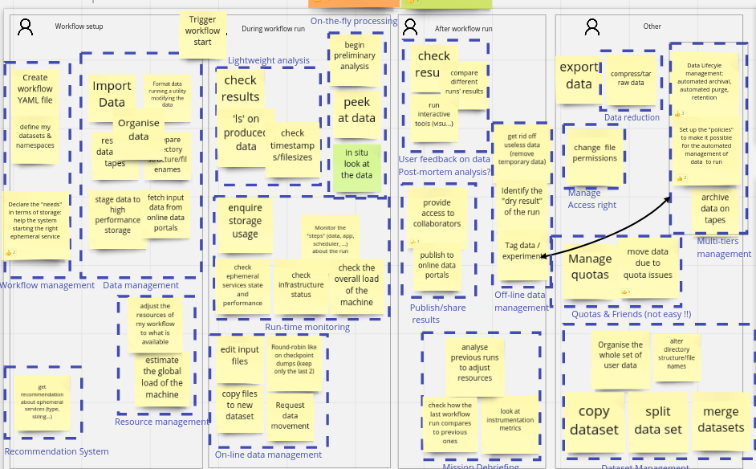
\includegraphics[width=0.75\textwidth]{FIGS/white-board.png}
    \caption[Co-design whiteboard]{ Screen capture of IO-SEA whiteboard co-design brainstorm session}
    \label{fig:white-board}
\end{figure}

Several key ideas came out from those co-design effort, in particular
\begin{itemize}
    \item \textbf{interactive data access:~} In all phases of the project, it is important for scientific use
    cases to have interactive access to the data sets and namespaces used in the workflow, e.g., to stage initial
    data in setup; to check output, peek at meta-data or even begin analysis while the workflow is running; to
    run interactive data analysis tools post-workflow.
    
    \item \textbf{Prompted tape archival/retrieval:~} The experience of scientific users at large HPC centres is
    that the time to move large datasets to or from tape can sometimes be measured in days. Therefore it is
    important that the users have an interface to trigger data retrieval from the tape long before a workflow is
    queued.
    
    \item \textbf{Tape-disk explicit copy:~} Much of the discussion regarding the IO-SEA storage hierarchy has
    used the phrase “data- movement”. As the tape archive is a tier in the storage hierarchy — the slowest but
    most capacious tier, use cases clarified that they rarely “move” data to or from the tape archive systems.
    This occurs normally only in response to suddenly needing to make space on a nearly-full disk. Rather the
    normal pattern is often that data is generated that has both near- term and long term uses and a copy is
    saved to tape for safe-keeping, while the bulk may remain on disk for further immediate access. Likewise,
    when older data is retrieved from tape for new analysis, it is usually copied to disk; the tape archive is
    not erased. This clarification has resulted in the inclusion of copy functionality of the datamover.
    
    \item \textbf{Pre-fetching to data node:~} Similarly, users in environments where compute-node time is
    charged against a budget ex- pressed concern that they be able to pre-fetch files to the data nodes so that
    the compute nodes do not idle when the allocation starts. Again, the solution provided in response was the
    datamovers, which will also allow users to prompt data movement to the flash storage. 
    
    \item \textbf{DASI-to-POSIX staging application:~} Several scientific use-case tasks expressed interest in
    exploring the proposed DASI as a method of organizing stored scientific data. However, to integrate DASI
    directly into the application generally requires significant re-writes to I/O libraries. In cases where the
    application is a large, widely-used community code, this is impractical and beyond the scope of the IO-SEA
    project. Instead, the use-case tasks have requested a stand-alone application that can translate a POSIX path
    to DASI semantic keys and copy a file back and forth between DASI and POSIX storage. This will enable us to
    explore the advantages of DASI with a low barrier to entry. Work Package~5 has indicated they intend to
    produce such an application in the coming months in response to this request. In anticipation of this,
    Section 5.1 provides an example of how this might be integrated into a workflow with the GBF ephemeral
    service.
\end{itemize}


\section{Outcomes from WP2}

The main outcomes from the second work package are related to the creation of the workflow manager. Since
ephemeral service are strongly associated to compute jobs, the following schema is to be respected
\begin{enumerate}
    \item allocate the compute nodes to run the simulation jobs
    \item allocate the data nodes in order to run the ephemeral services
    \item start the ephemeral services
    \item make the ephemeral services accessible to the compute nodes, for example mounting a NFS share
    exposed via a NFS ephemeral service
    \item run the simulation
    \item if several steps are involved in the simulation, run the other steps of the simulation
    \item end the simulation
    \item flush the data to the persistent storage (typically the object stores)
    \item stop the ephemeral services
    \item release the data nodes and the compute nodes
\end{enumerate}

The WP2 made all the development to achieve this schema. The main outcome developed in the Workflow manager,
which makes it possible to manage the allocation of temporary IO servers, or ephemeral servers, implemented in 
the IO-SEA. As compute jobs are running on compute nodes, ephemeral services are working on data nodes, which
are part of dedicated modules within the MSA (see \ref{fig:msa}). 

The Workflow Manager operates as described in figure \ref{fig:wfm}. The concept of compute job is replaced by
the more complete concept of workflow. A workflow is made of different steps, where simulation program are run
as well as ephemeral service. 

\begin{figure}[H]
    \centering
    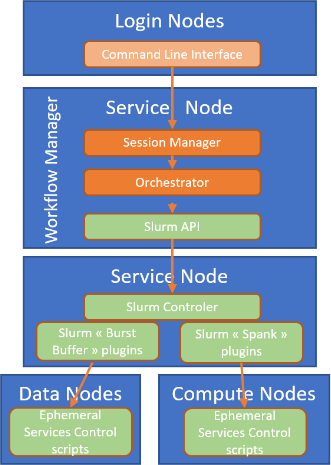
\includegraphics[width=0.35\textwidth]{FIGS/wfm.png}
    \caption[Worflow Manager Architecture]{ Worflow Manager Architecture}
    \label{fig:wfm}
\end{figure}

The workflow contains explicit dependencies, for example you need to have an
already started ephemeral IO server before you can do actual IO operations. The workflow is described by a 
workflow description file, written in JSON. 

The Workflow Manager is a key component inside the IO-SEA, it's a central place where all pieces are set
together. The user requirements from WP1 drove most of the development of this feature and operated in clode
collaboration with WP2. The WFM starts and uses the ephemeral servers developed by WP4 as well as elaborated
user interfaces provided by WP5. 

Inside the Workflow Manager resides an orchestrator whose tasks is to allocate and start all the executables
involved in a workflow. From this perspective, the orchestrator has strong acquaintance with the compute center's
resource scheduler (such as Slurm). The figure \ref{fig:it4i} showns how such a framework was deployed on the 
OpenStack Cloud hosted at IT4I, it is an actual proof that the workflow manager actually works. 

\begin{figure}[H]
    \centering
    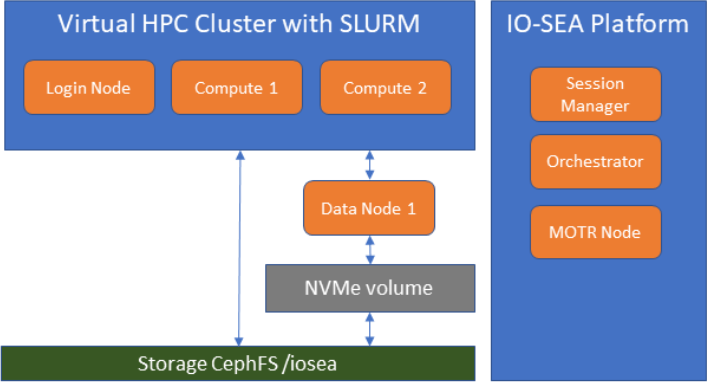
\includegraphics[width=0.75\textwidth]{FIGS/it4i.png}
    \caption[Worflow Manager at IT4I]{Instances deployed at IT4I OpenStack Cloud}
    \label{fig:it4i}
\end{figure}

The Workflow manager comes with itw own API and a set of command-line utility that help in efficiently manage
the workflow related operations (such a "start" / "stop" or "pause" / "resume"). 


\section{Outcomes from WP3}

The third Work Package of the IO-SEA project makes a focus on instrumentation and monitoring, plus the
development of tools to extract useful bits of information from the collected data. 

During the three years run of IO-SEA, WP3 has succeeded in developing a fine instrumentation framework able to
get hardware and software probes. In particular, the WP3 utility makes it possible to observe and measure the 
behavior of applications. By having a fine understanding of the mechanisms involved in the different core
components of IO-SEA, mostly used in WP2 and WP4. This makes it possible to put probes at the exact right 
location, exposing quite relevant data.

\begin{figure}[H]
    \centering
    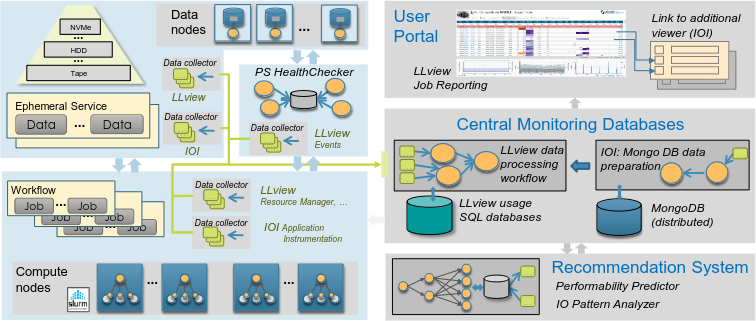
\includegraphics[width=0.75\textwidth]{FIGS/io_instr.png}
    \caption[I/O Monitoring architecture]{ The Architecture of the I/O monitoring framework}
    \label{fig:instr}
\end{figure}

This data is collected in databases, and can be later displayed via interactive 
GUI. Such integration as for example been done in tools via LLView or ParaStation HealthChecker. Giving a clear
overview is interesting, but this is not the only benefit of WP3, the instrumentation databases are dug via 
AI framework in order to build a \textit{recommendation system}. This new feature helps in identifying patterns
in the user application, opening the path to optimising those applications. Within the scope of the IO-SEA
project, such a recommendation systems could automatically add "hints" on objects or datasets, helping WP4 and
the HSM feature capable of using this hints as an input in their internal policies.

\begin{figure}[H]
    \centering
    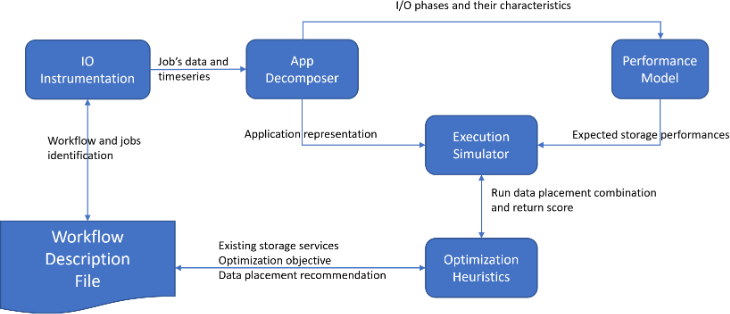
\includegraphics[width=0.75\textwidth]{FIGS/recom.png}
    \caption[Recommendation system]{ The general architecture of the recommendation system}
    \label{fig:recom}
\end{figure}

A side effect of this work is the "IO Traces Collection" initiative supported by both projects, ADMIRE and
IO-SEA. This initiative offers a non intrusive instrumentation framework whose well formatted output should be
stored in a common database, hosted on the internet and available to everyone. Researchers could use this tool
to work on optimisation for they have a large zoo of many different application behaviors. 





\section{Outcomes from WP4}

Several outcomes come from the WP4. During the three years of the project, it became obvious that a clear 
management of a generic HSM made it necessary to have a defined API and a defined architecture. This API, name HESTIA (ADD MEANING OF THE ACRONYM), make this possible. HESTIA is not attached to any feature of a given object 
store. In IO-SEA, it brings all the tools needed to implement the HSM feature between Phobos and another object
store.

The HESTIA API models and formalises ways to use various storage technologies  like NVMe, SSD, HDD, or tape, to
allow object stores to handle every type of device within the same storage hierarchy. It will make IO-SEA 
capable of dealing with the complete lifecycle of the data inside the same system. This system will be capable of managing most of the existing storage devices, from NVMe to tapes. To achieve this, it leverages two open-source
object stores: CORTX-Motr on top of Phobos (with the necessary abstractions to support additional backends).
Thus, HSM mechanisms are implemented in two products, making them capable of managing data movements between
them. The figure \ref{fig:hestia} depicts how the different compoments are organised within the HESTIA 
framework. 

\begin{figure}[H]
    \centering
    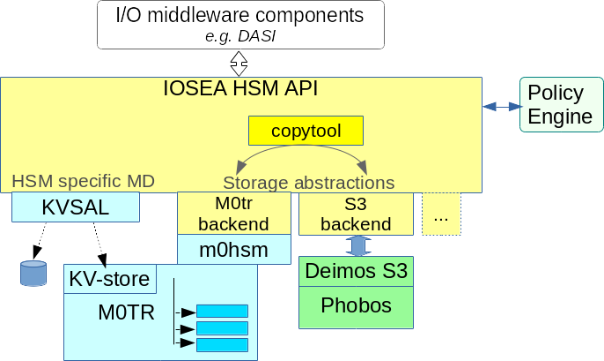
\includegraphics[width=0.75\textwidth]{FIGS/hestia.png}
    \caption[HESTIA software architecture]{ The architecture of the HESTIA framework}
    \label{fig:hestia}
\end{figure}

Hestia is an open source project that can be found at \url{https://git.ichec.ie/io-sea-internal/}.

HESTIA manages the data movement and triggers some of them internally (e.g. for managing data migration as data
have become cold enough to be migrated to tapes). The Robinhood software (available at
\url{https://github.com/cea-hpc/robinhood}, is the policy engine used to achieve that goal. 

PHOBOS, or \textit{Parallel Heterogeneous OBject Store}, is an object store developed at CEA and available as an
open-source software at \url{https://github.com/cea-hpc/phobos}. PHOBOS existed before the beginning of IO-SEA,
but was strongly improved during the three years of the project. PHOBOS is designed to manage large volumes of
data for various kinds of storage technologies from SSD to tapes. Phobos can efficiently handle very large
datasets on inexpensive media without sacrificing scalability, performance, or fault-tolerance requirements.

Phobos is designed to allow the easy integration of new modules for layouts such as mirroring and erasure coding
or I/O adapters. It's architecture can be seen on figure \ref{fig:phobos}. 

\begin{figure}[H]
    \centering
    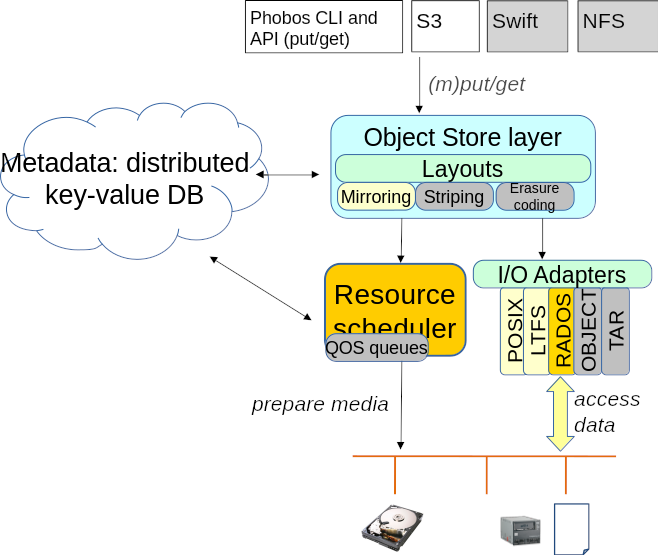
\includegraphics[width=0.75\textwidth]{FIGS/phobos.png}
    \caption[PHOBOS architecture]{ The architecture of the PHOBOS software}
    \label{fig:phobos}
\end{figure}

KVSNS is a library that makes it possible to implement a POSIX semantic on top of the services provided by an
object store and a key-value store. KVSNS was originally developed in the run of the SAGE and SAGE2 project, but
the related version was not capable of managing object store with only a CRUD\footnote{Create Read Update Delete}
interface, the object store had to be capable of performing random I/O operations in objects, just like POSIX
does via the \verb|pread()| or \verb|pwrite()| from the LibC. Inside IO-SEA, KVSNS gain a new feature, making it
capable of dealing with CRUD-only obbject store. This required the introduction of a local filesystem used as
a cache and a way to fetch and dispose entry from/to this cache. This logic should not be a bottleneck, it should
be implemented as a fully parallel and distributed service. This lead to the development of the GRH feature.
It's layers are described by figure \ref{fig:kvsns}

\begin{figure}[H]
    \centering
    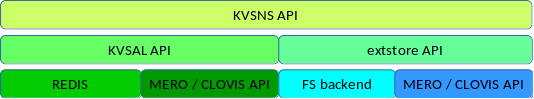
\includegraphics[width=0.75\textwidth]{FIGS/KVSNS_architecture.png}
    \caption[KVSNS layers]{ The layers of the KVSNS library}
    \label{fig:kvsns}
\end{figure}

GRH gets request issued by the KVSNS library itself, or externally. It creates an asynchronous request id that
can be used by the client to get the status of the request in an asynchronous way. GRH implement workers and 
tasks queues. GRH is based on the Celery framework, which is strongly parallel. GRH could be used outside its
original scope.In particular, GRH can be used to implement a data mover. The overall architecture of the GRH is
described by figure \ref{fig:grh}. 

\begin{figure}[H]
    \centering
    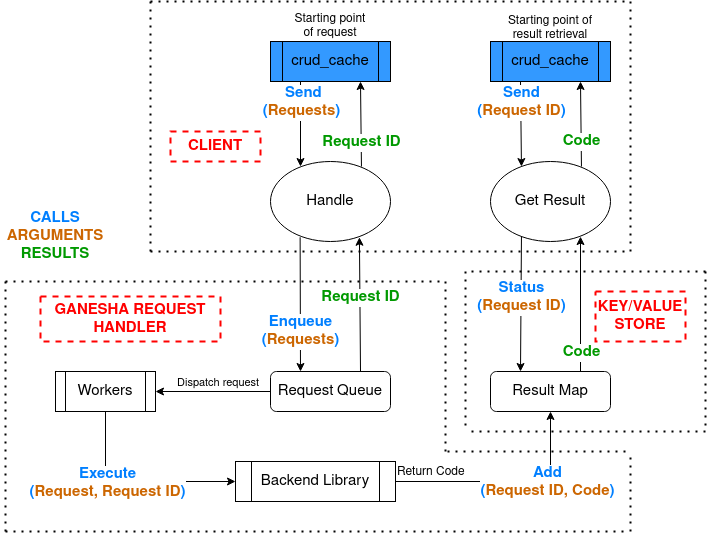
\includegraphics[width=\textwidth]{FIGS/GRH.png}
    \caption[GRH architecture]{ The design of the GRH component}
    \label{fig:grh}
\end{figure}

IO-SEA strongly relies on object stores. Implementing the IO-SEA architecture from scratch is easy, as new
data will be inserted inside directly in the object store, but what about moving data, already stored in standard
distributed and parallel file-systems? It's important to implement the required tools to make it possible to 
migrate data from the previously existing storage systems. One of the promises in the IO-SEA's proposal is 
providing such a framework. This goal was actually achieved as shown in figure \ref{fig:migration-path}. 

\begin{figure}[H]
    \centering
    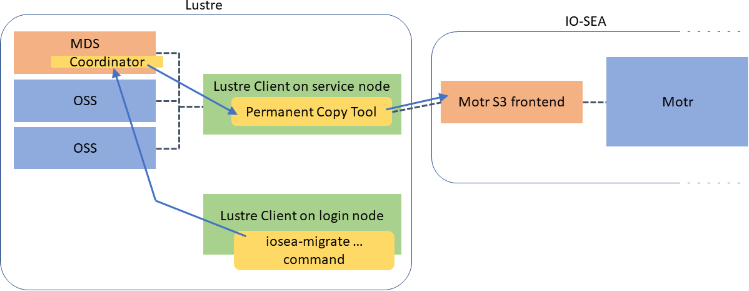
\includegraphics[width=0.75\textwidth]{FIGS/migration-path.png}
    \caption[Migration Path]{ The migration path in the IO-SEA}
    \label{fig:migration-path}
\end{figure}

\section{Outcomes from WP5}

The main outcome of the WP5 is the \textit{Data Access Storage Interface}, or \textbf{DASI}. 
DASI (available at \url{https://github.com/io-sea/dasi}) is a semantic interface for data, where the data is
indexed and uniquely identified by sets of scientifically-meaningful metadata keys. DASI is modular and is
compatible with multiple backends (i.e., object stores or POSIX) through diverse frontends (Python, C++, C).

Internally, DASI is based on software developed by ECMWF, named FDB2, which has been developed in previous EU
projects (NEXTGenIO), but has been heavily adapted and extended to be agnostic of and configurable for
different scientific domains. Leveraging FDB in this way means that many backends are already supported by DASI,
including a high-performance POSIX backend, a Ceph object storage backend, and an NVRAM backend. During the
IO-SEA project, a backend will also be created for CORTX. Applications will have seamless access to these
backends once they have been modified to support DASI. The DASI architecture is shown in figure \ref{fig:dasi}
as well as its dependency to other work done in the scope of IO-SEA.

\begin{figure}[H]
    \centering
    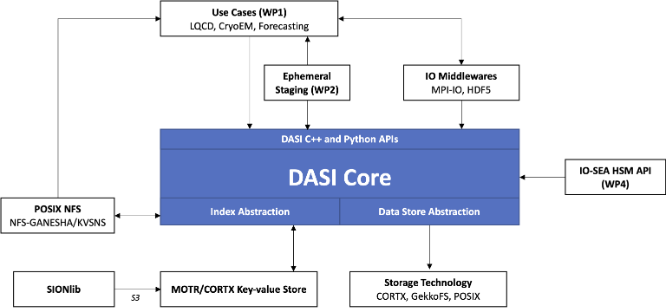
\includegraphics[width=0.75\textwidth]{FIGS/dasi.png}
    \caption[Migration Path]{ DASI and its interactions with the other elements of IO-SEA}
    \label{fig:dasi}
\end{figure}

DASI is domain-agnostic, and is configured for each scientific domain using a schema. The schema
defines the metadata keys which index and identify the data within a domain. 

\paragraph{}
DASI comes with a specific libraty and its own API, but it includes a POSIX interface based on the KVSNS
library and the nfs-ganesha server. It is interface with existing middleware like SIONlib, but it has 
dedicated interfaces to standards like MPI or HDF5. 





	%%%%%%%%%%%%%%%%%%%%%%%%%%%%%%%%%%%%%%%%%%%%%%%%%%%%%%%%%%%%%%%%%
	%%%%%%%%%%%%%%% put in a glossary %%%%%%%%%%%%%%%%%%%%%%%%%%%%%%%
	\printglossary[title={List of Acronyms and Abbreviations}]

	%%%%%%%%%%%%%%%%%%%%%%%%%%%%%%%%%%%%%%%%%%%%%%%%%%%%%%%%%%%%%%%%%
	%%%%%%%%%%%%%% put in References %%%%%%%%%%%%%%%%%%%%%%%%%%%%%%%%
	\bibliographystyle{unsrt}
	\bibliography{Postamble/IO-SEA}

\end{document}
